\documentclass[t]{beamer}
\usetheme[deutsch]{KIT}
\setbeamercovered{transparent}
\setbeamertemplate{navigation symbols}{}
\graphicspath{ {Systemmodelle/images_blank/} }

\KITfoot{ Croggle - Praxis der Softwareentwicklung WS 13/14}
\usepackage[utf8]{inputenc}
\usepackage{ngerman}
\usepackage[scaled]{uarial}
\renewcommand*\familydefault{\sfdefault}
\usepackage[T1]{fontenc}
\usenavigationsymbols


\usepackage{listings}
\usepackage{xcolor}




\title{Croggle}
\subtitle{PSE - Entwurfsphase \\[0.3cm]
Lukas Böhm $\cdot$ Tobias Hornberger $\cdot$ Jonas Mehlhaus \\ Iris Mehrbrodt  $\cdot$ Vincent Schüßler $\cdot$ Lena Winter}
\institute[IPD]{Institut für Programmstruktutren und Datenorganisation}

\TitleImage[height=\titleimageht]{banner.png}


\begin{document}

\begin{frame}
        \maketitle
\end{frame}

\begin{frame}
	\frametitle{Designentscheidungen}
	Wegweisende Entscheidungen für den weiteren Aufbau der App:\\
	\begin{itemize}
		\item Model View Controller
		\item libgdx
		\item Aufbau des Model
		\item Visitor Pattern
		\item Levelrepräsentation mit JSON
		\item SQLite Datenbank
		\item Observer/Listener Pattern
	\end{itemize}
	%%\includegraphics<1>[width=0.85\textwidth]{mvc.jpg}

	%%\includegraphics<2>[width=0.8\textwidth]{libgdx.png}
\end{frame}

\begin{frame}
	\frametitle{Nicht umgesetzte Wunschkriterien}
	Nicht modellierte Wunschkriterien, die nicht weiter verfolgt werden: \\
	\begin{itemize}
		\item Avatarerstellung (/F130+/)
		\item Automatische Kameraführung (/F236+/)
		\item Bestimmte Achievements (/F250+/)
		\begin{itemize}
			\item Nichtterminierender Ausdruck
			\item Anzahl Spalten/Zeilen
			\item Erreichtes innerhalb einer Spielsitzung
		\end{itemize}

		\item Sandboxlevel speichern/laden (/F260+/)
	\end{itemize}
\end{frame}

\begin{frame}
	\frametitle{Repräsentation der \(\lambda\)-Terme}
	\begin{center}
		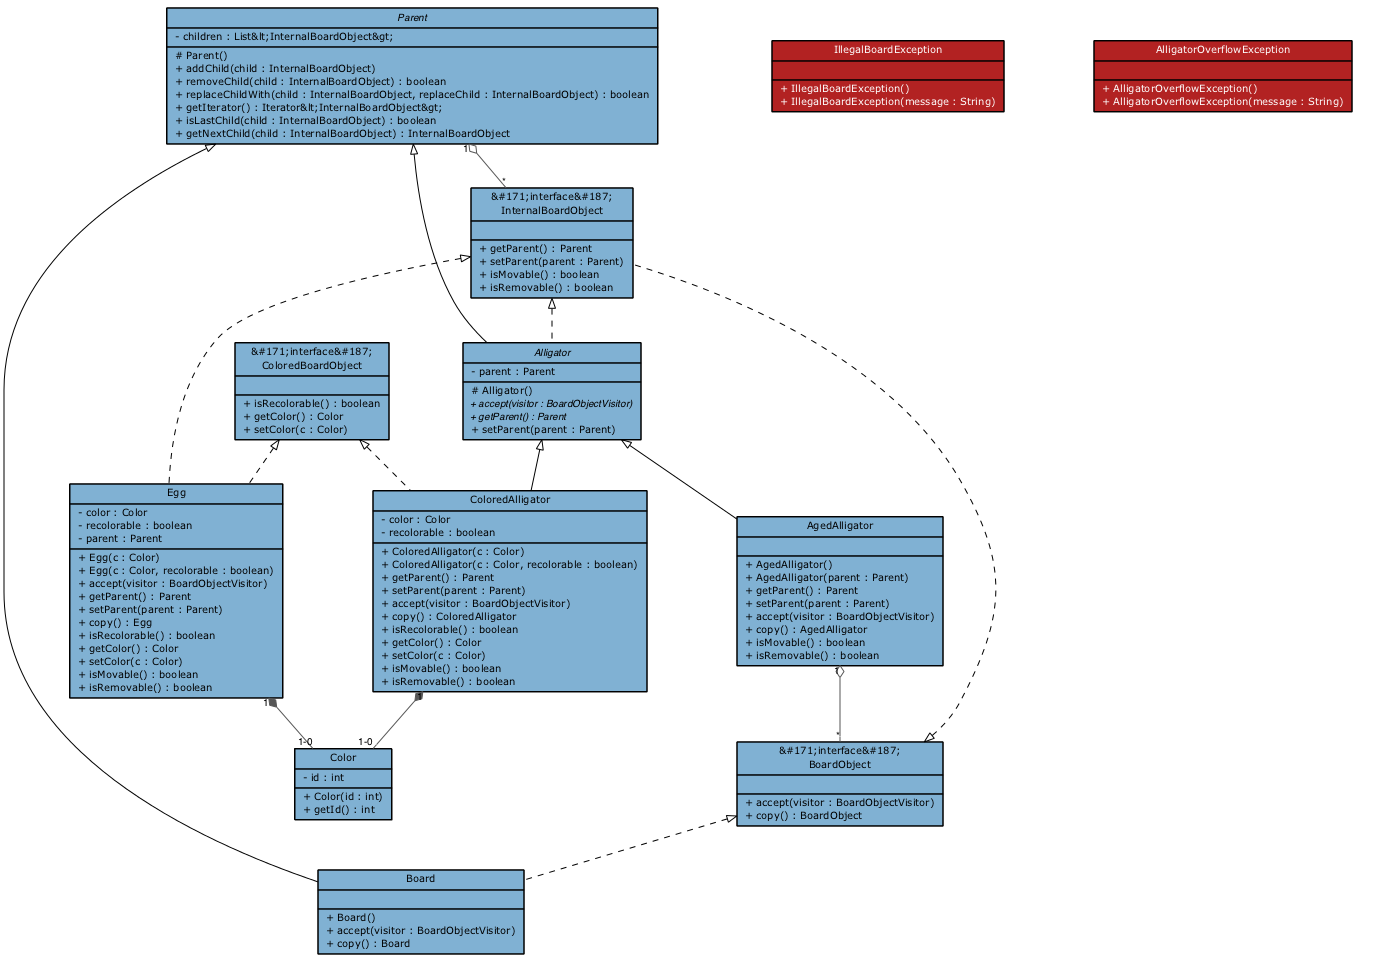
\includegraphics[width=0.8\textwidth]{umlAwesome.png}
	\end{center}
\end{frame}

\begin{frame}
	\frametitle{Sequenzdiagramm \(\beta\)-Reduktion: (\(\lambda\)x.x) y}
	\begin{center}
	\includegraphics<1>[width= 0.4\textwidth]{Alligator1.png}
	\includegraphics<2>[width=0.5\textwidth]{Beta-Reduktion.png}
	\end{center}
\end{frame}

\begin{frame}
	\frametitle{Call-by-Name Anwendung}
	\begin{center}
	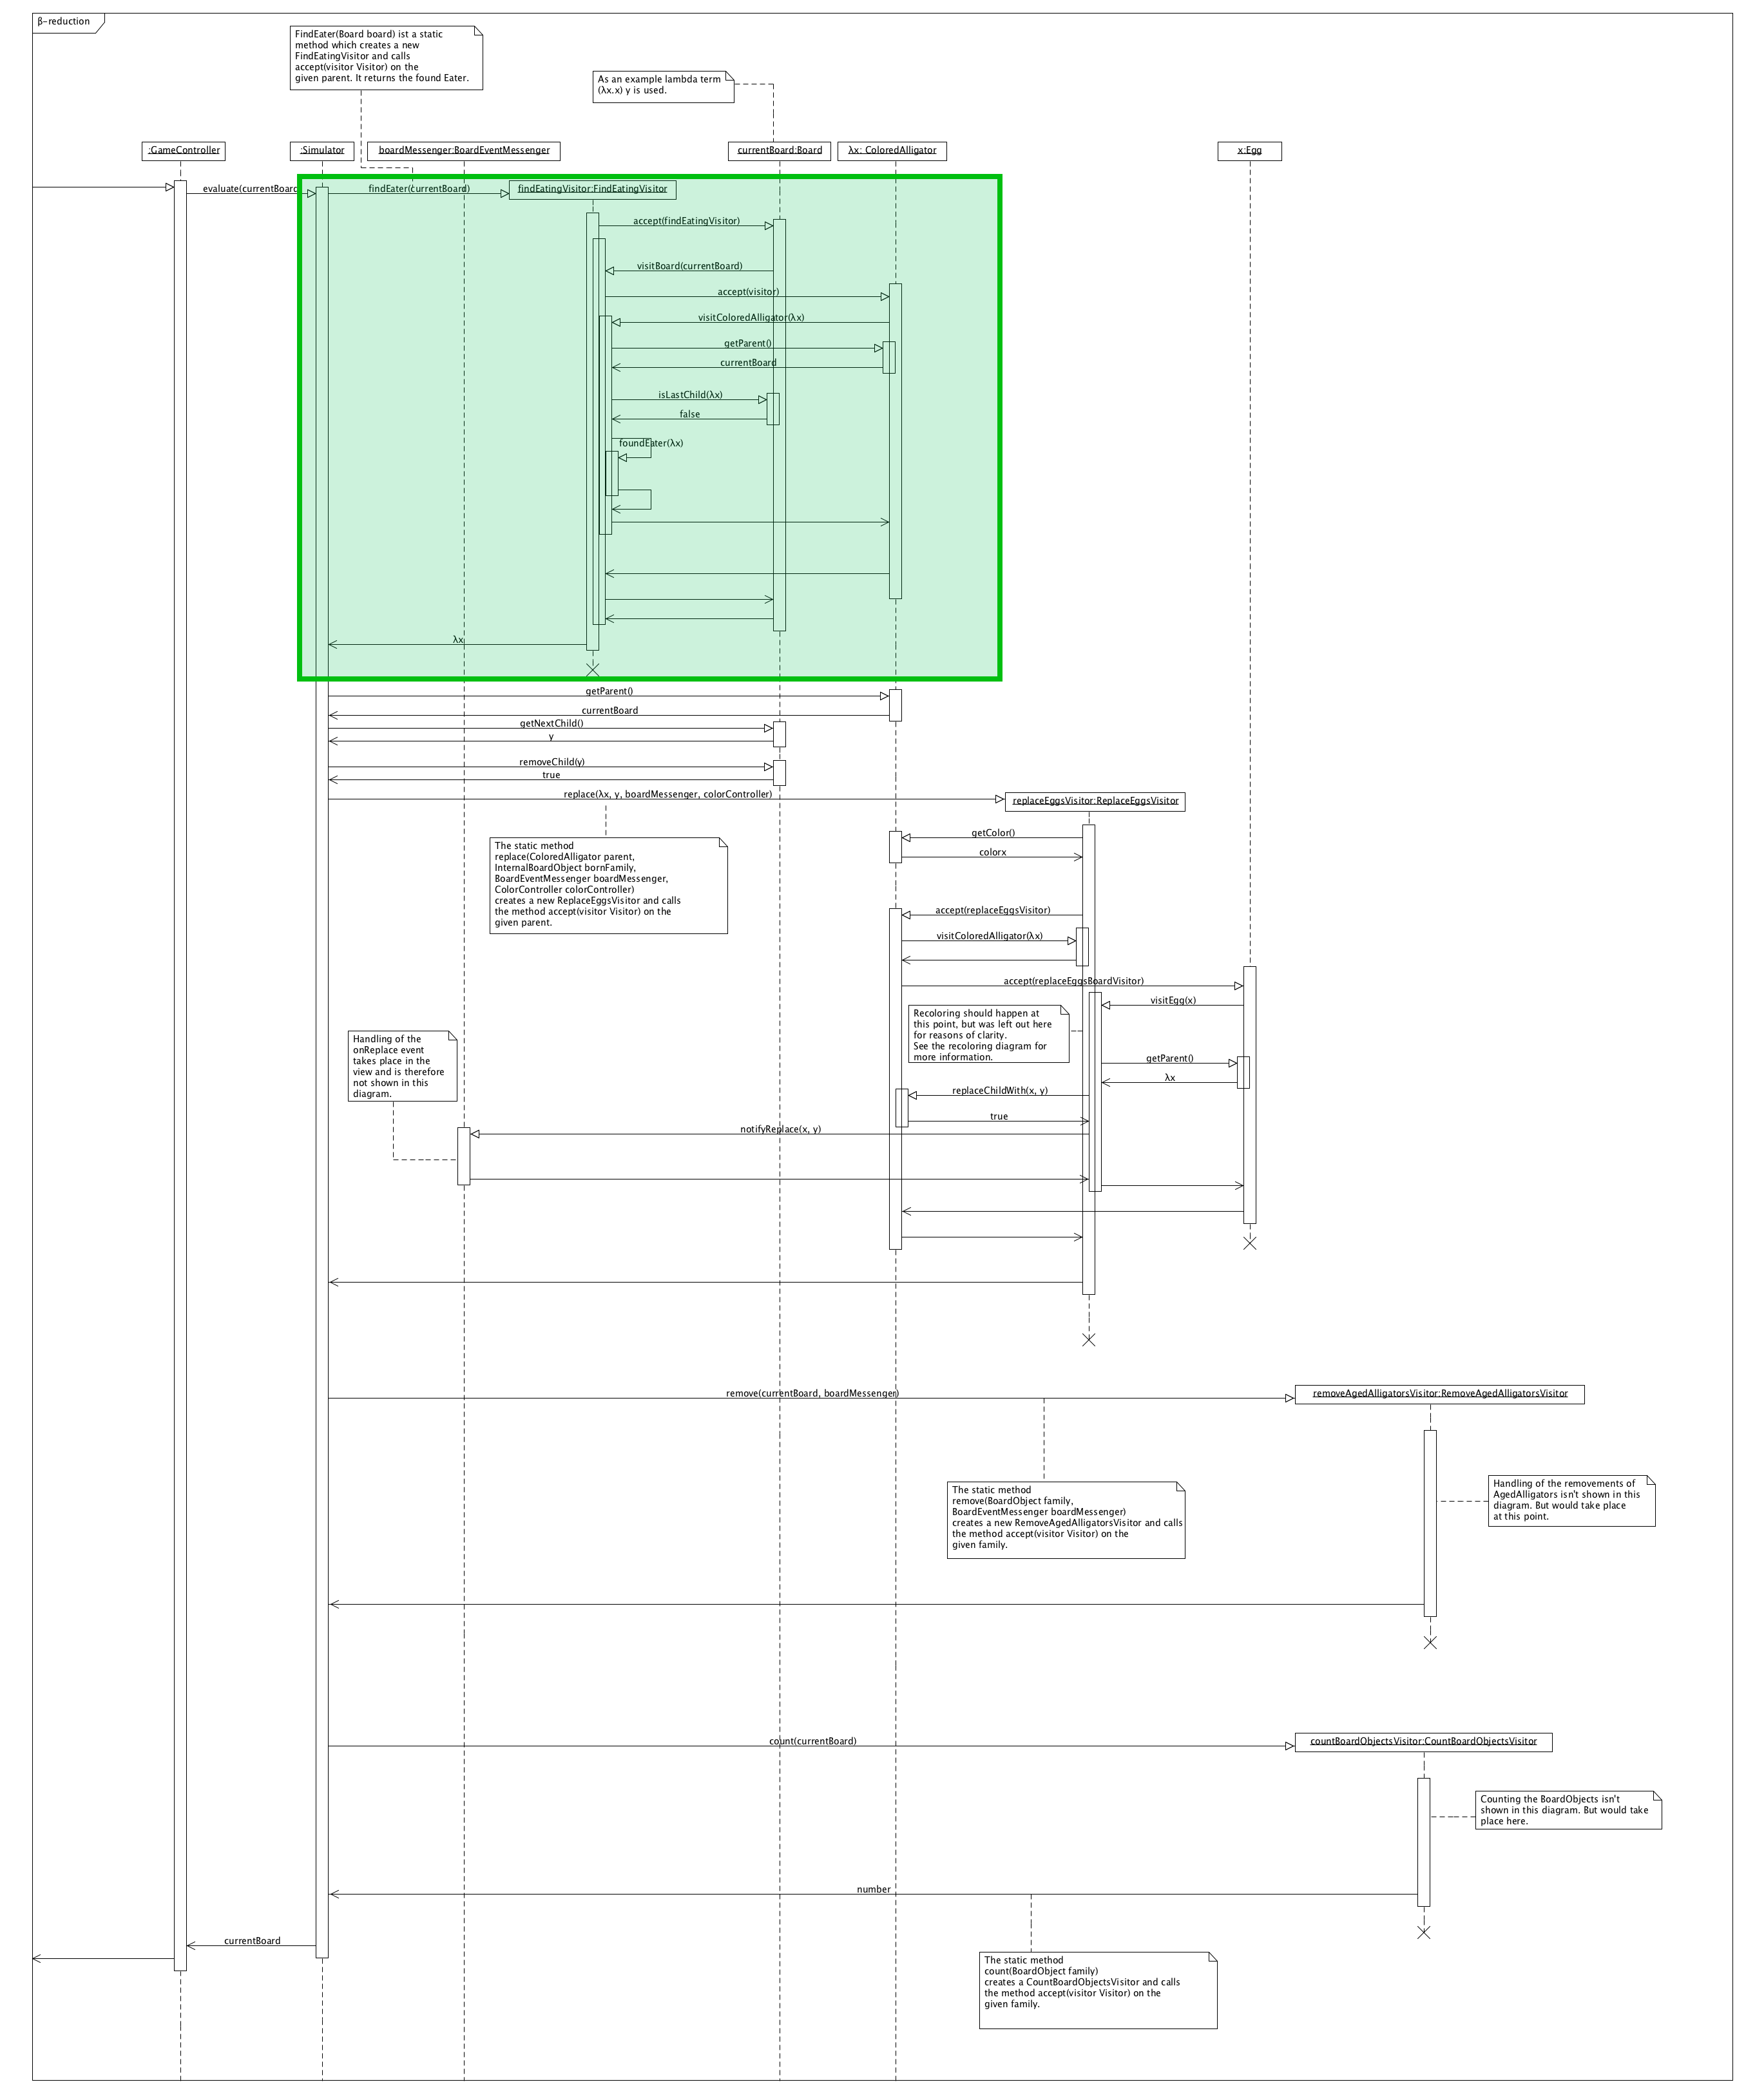
\includegraphics[width=0.5\textwidth]{Beta-Reduktion-withGreen.png}
	\end{center}
\end{frame}

\begin{frame}
	\frametitle{Call-by-Name Anwendung: Detailansicht}
	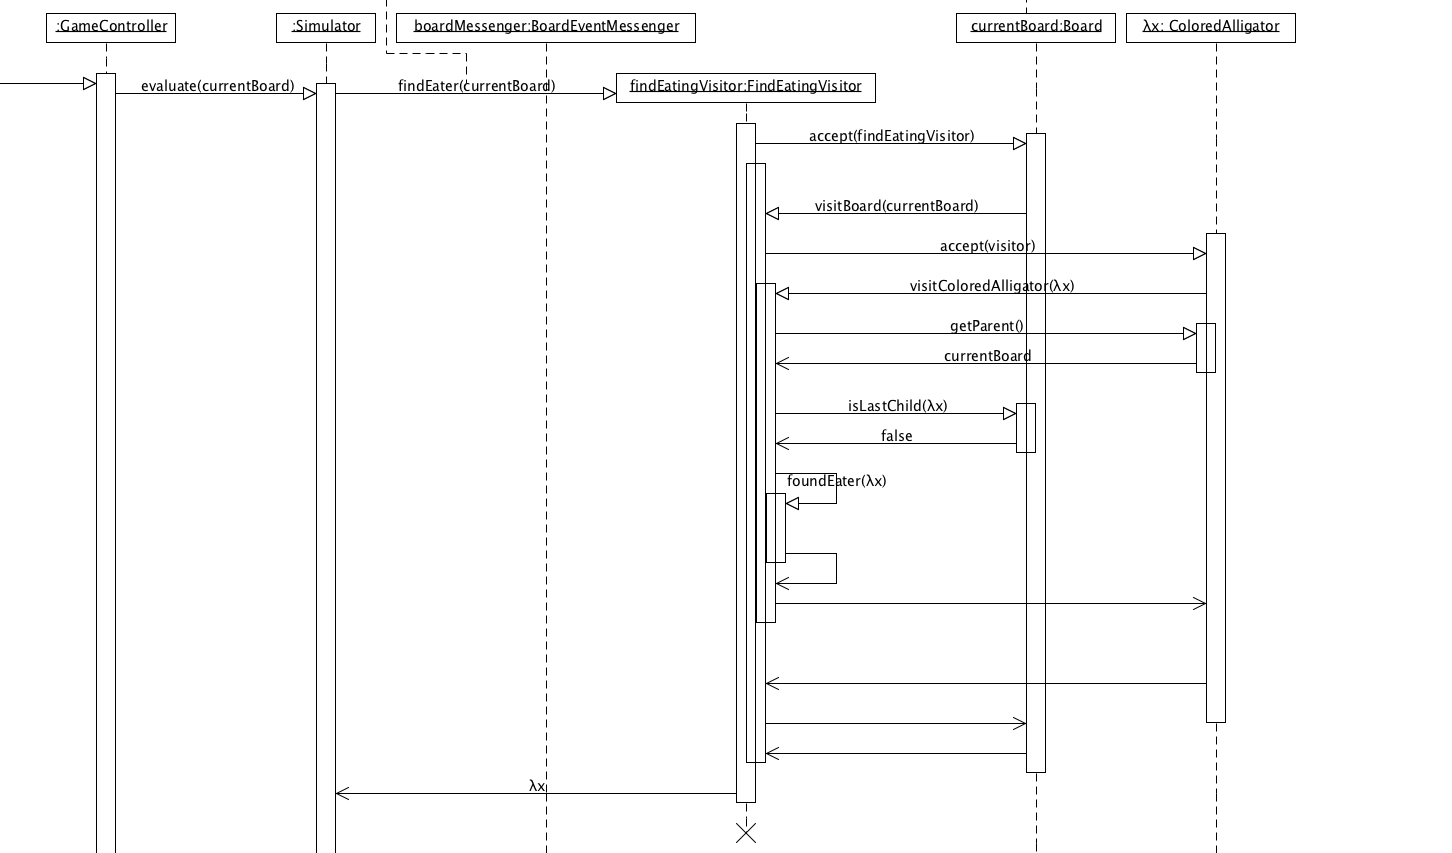
\includegraphics[width=\textwidth]{FindLocation.png}
\end{frame}



\begin{frame}
	\frametitle{Änderungen im Baum}
	\begin{center}
		\includegraphics<1>[width=0.5\textwidth]{Beta-Reduktion-withBlue.png}
	\end{center}
\end{frame}

\begin{frame}
	\frametitle{Änderungen im Baum: Detailansicht}
	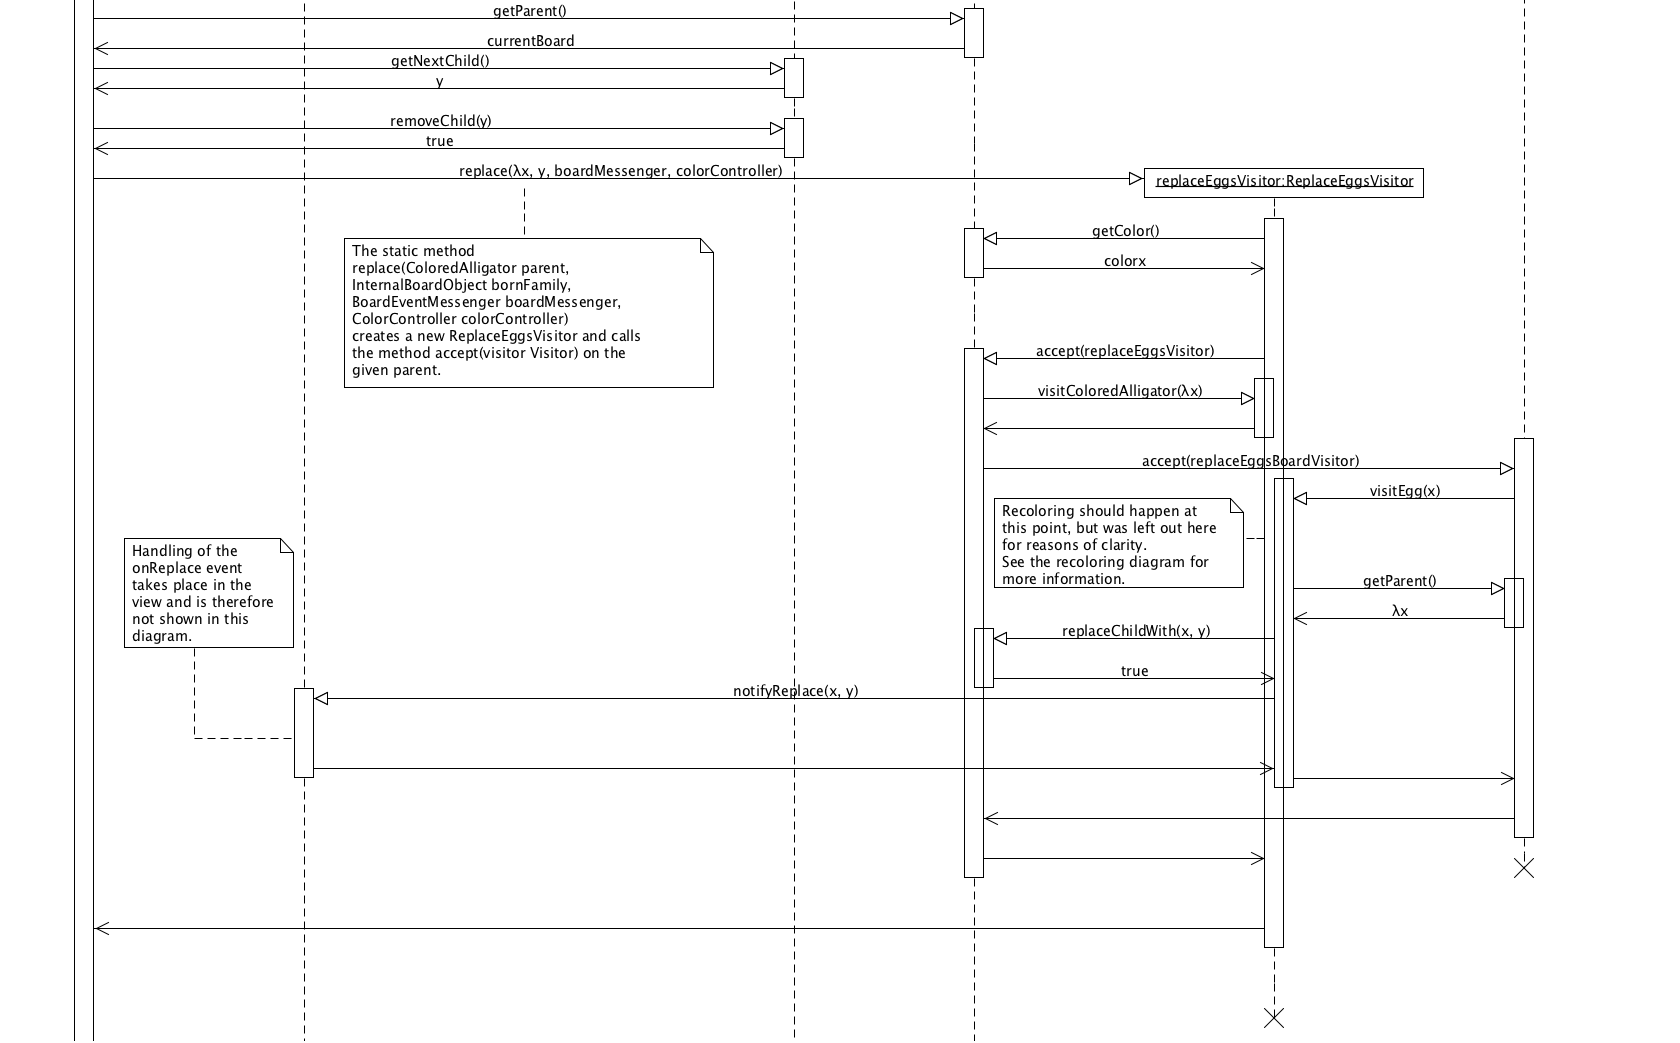
\includegraphics[width=0.95\textwidth]{ReplaceEggs.png}
\end{frame}

\begin{frame}
	\frametitle{Spielbrett aufräumen}
	\begin{center}
		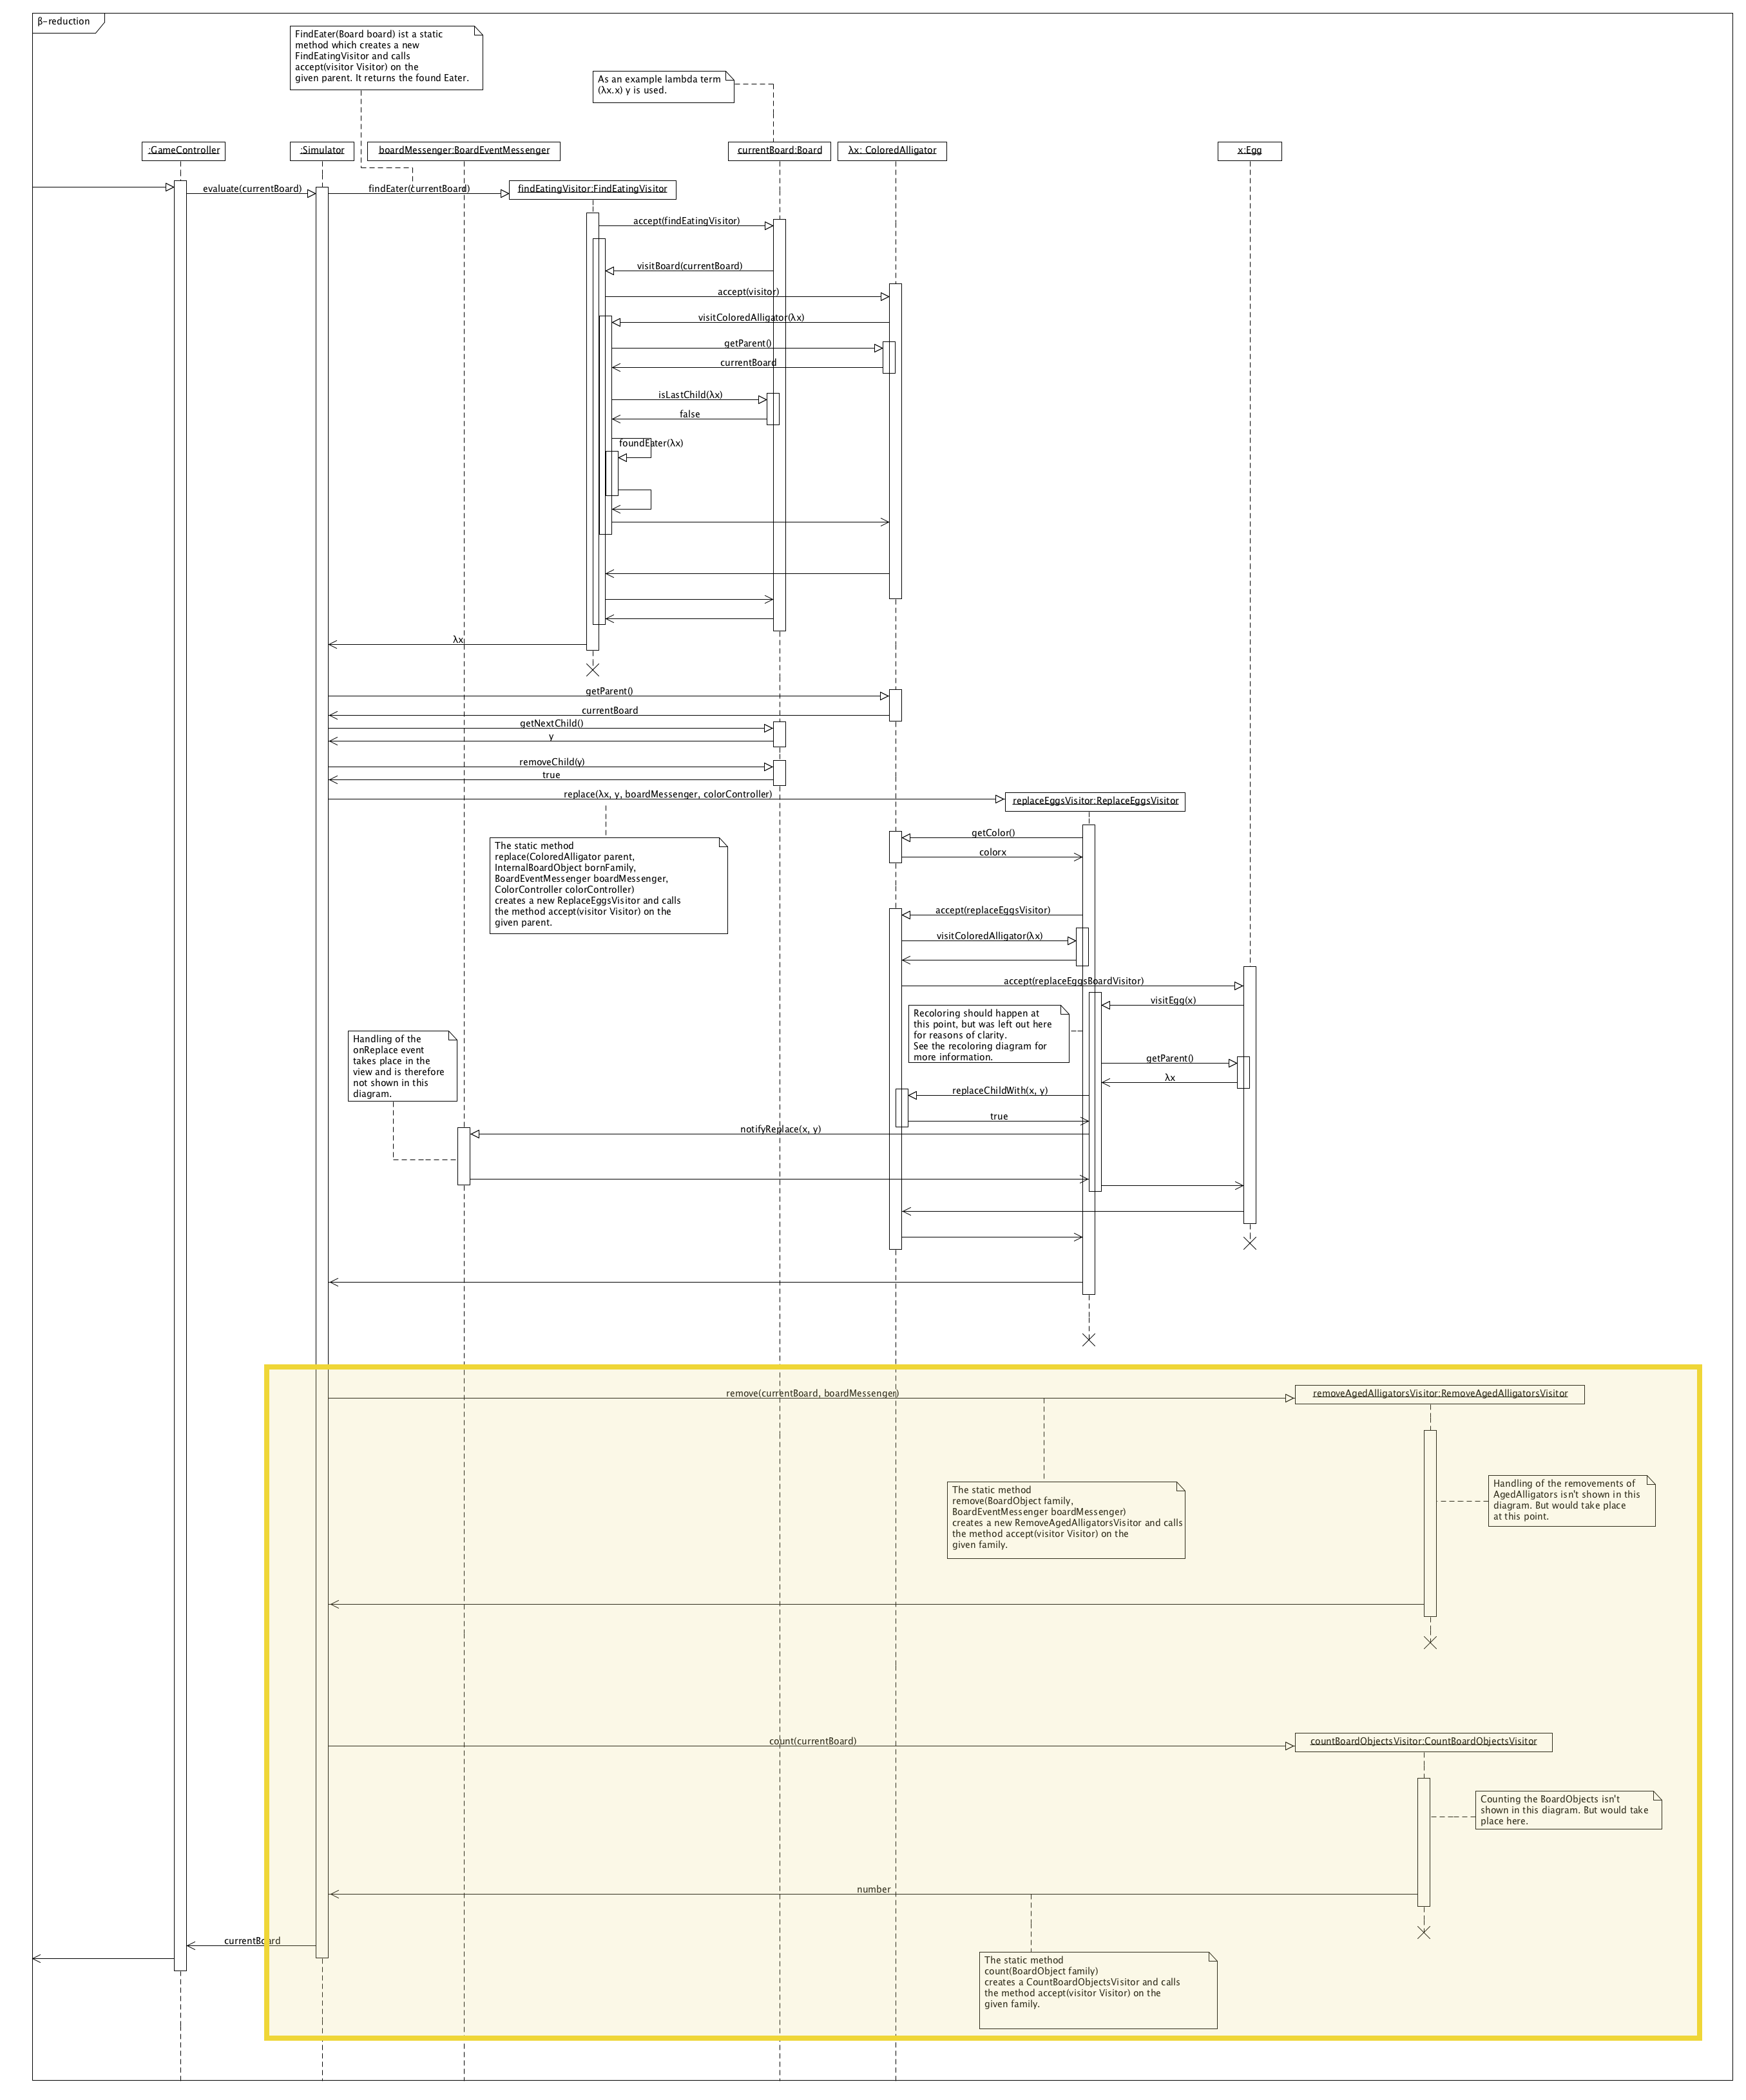
\includegraphics[width=0.5\textwidth]{Beta-Reduction-withYellow.png}
	\end{center}
\end{frame}

\begin{frame}
	\frametitle{Ergebnis}
	\begin{center}
		\includegraphics[width=0.4\textwidth]{Alligator2.png}
	\end{center}
\end{frame}

\begin{frame}
	\frametitle{}
	\begin{center}
	\begin{Huge}
		Vielen Dank\\ für Ihre Aufmerksamkeit
	\end{Huge}
	\end{center}
\end{frame}

%%\begin{frame}
%%	\frametitle{\(\beta\)-Reduktion: Detailansicht}
%%	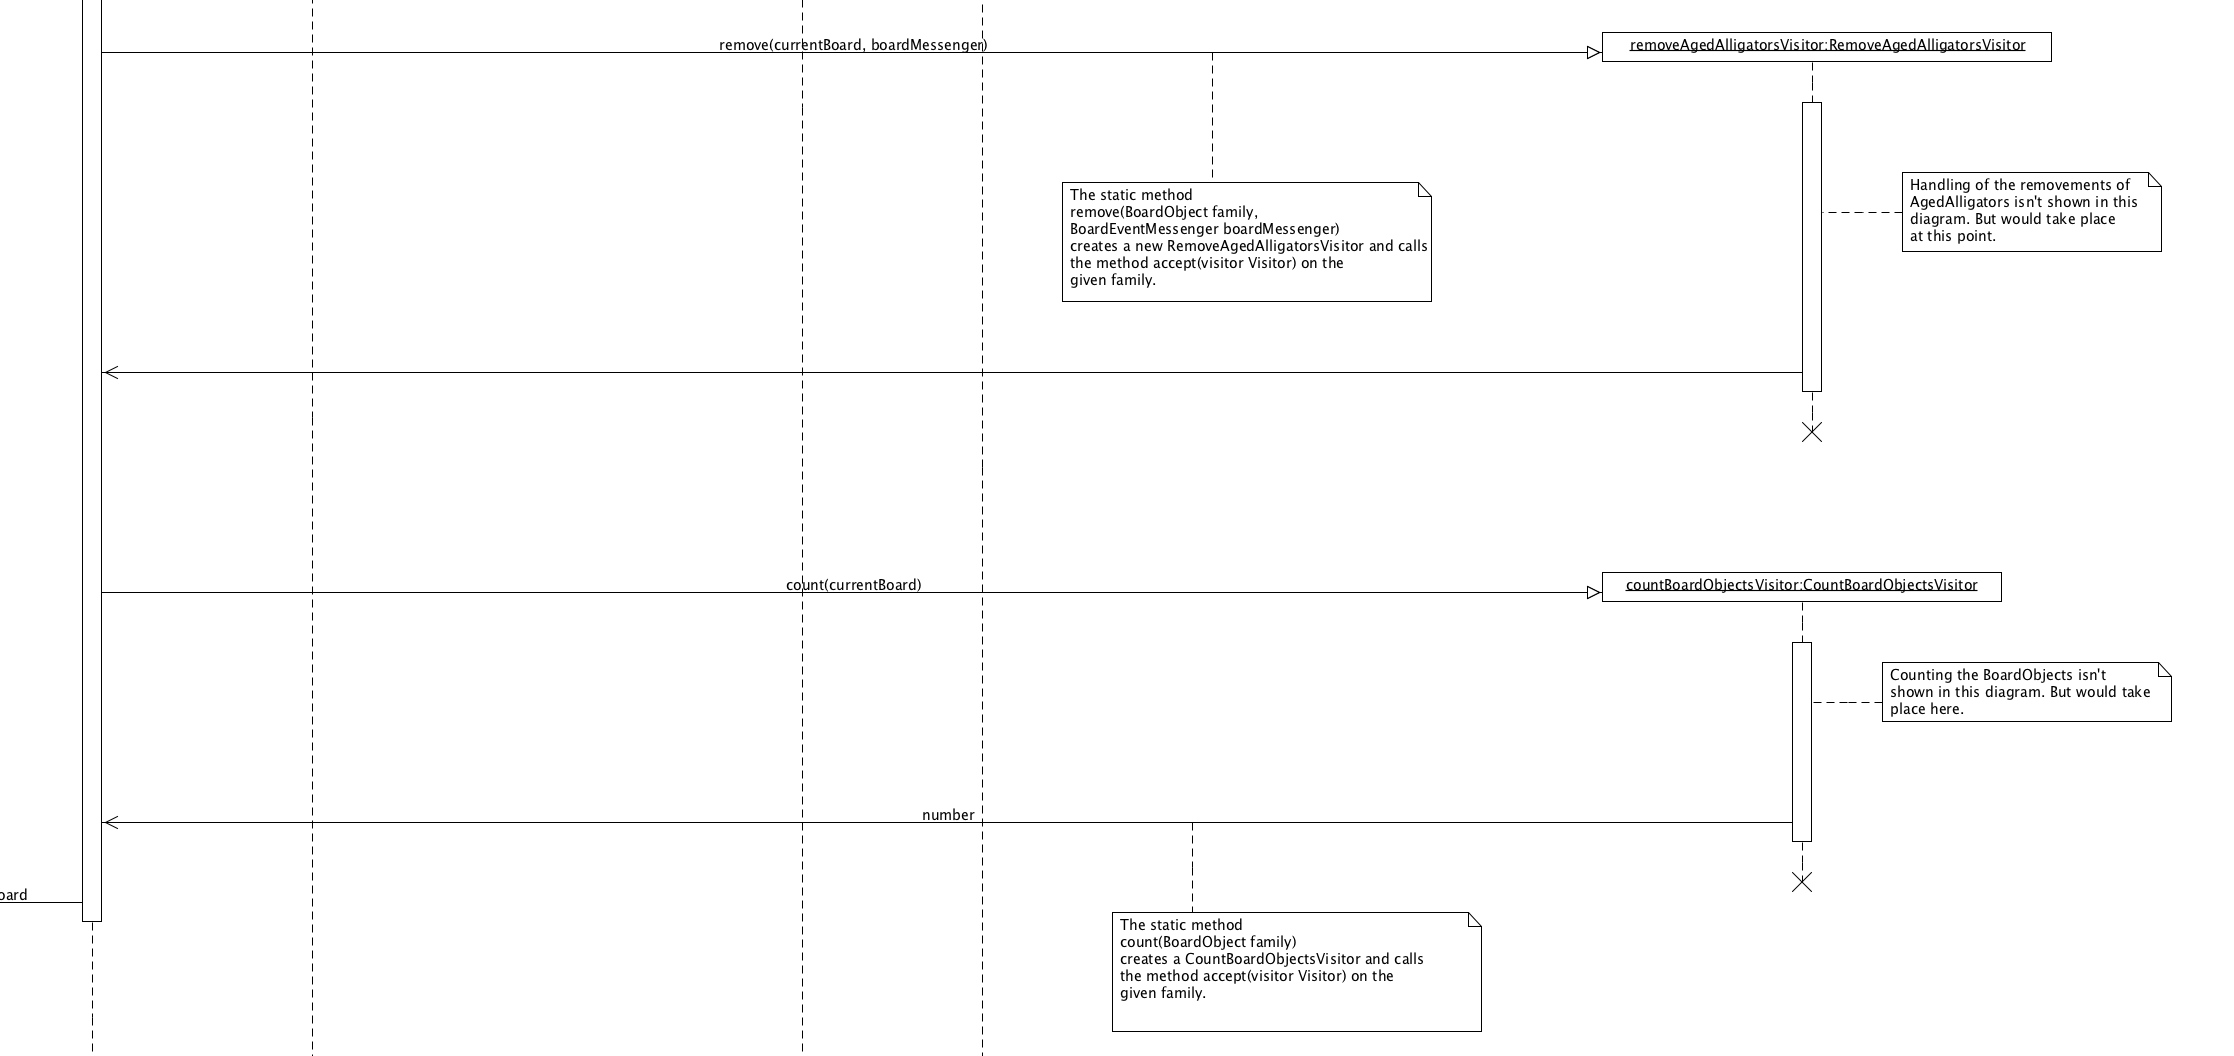
\includegraphics[width=\textwidth]{unnoetig.png}
%%\end{frame}

\end{document}
